\chapter{Experimenty}\label{ch:experimenty}

%Podrobnější popis sledovaných dat.

Po křižovatce požadujeme, aby zaručovala bezpečnou cestu autům.
Nyní budu předpokládat, že agenti dávají přesnou informaci křižovatce a plně dodržují plán.
Za tohoto předpokladu nám algoritmus zaručuje nekolizní trasy.

Následujícím faktorem je zpoždění aut.
Budu sledovat \hyperref[par:zamitnuti]{počet zamítnutých agentů} a \hyperref[par:zdrzeni]{zdržení} naplánovaných agentů.
V tabulkách budu porovnávat celkový \hyperref[par:zamitnuti]{počet zamítnutých agentů} (Zam).
U \hyperref[par:zdrzeni]{zdržení} budu počítat celkový součet (Zpož)
a průměrné \hyperref[par:zdrzeni]{zdržení} na agenta (pZp) vypočítané ze všech agentů.

Další zajímavý faktor je obsazenost křižovatky,
který udává v kolika krocích ze všech byl některý agent na určitém bloku křižovatky.
Ve výsledkách budu počítat průměrný počet agentů na křižovatce (pAg) přes všechny kroky.
%Budu také sledovat průměrnou délku naplánovaných cest. TODO

Důležitá je také doba běhu algoritmu.
Budu sledovat pro každý krok, kolik uběhlo času od spuštění plánování daného kroku.
Odtud zpočtu průměrný čas na jeden krok v milisekundách (Čas).

Nejprve provedu testy pro porovnání parametrů jednotlivých agentů.
Poté srovnám nejlepší nastavení algoritmů proti sobě.
%V poslední sekci zavedu k agentům určité nepřesnosti, které můžou způsobit kolize.
%Poté budu pozorovat vliv těchto nepřesností na počet kolizí u jednotlivých algoritmů.


\section{Testovací data}\label{sec:testovaci_data}

%Popis experimentálních dat - velikost křižovatky, počet agentů a kroků, safe distance.

\subsection{Délka simulace}\label{subsec:delka_simulace}

Simulace bude přidávat agenty po $32768$ kroků.
Pokud bude plánování trvat příliš dlouhou dobu, bude simulace předčasně ukončena.
Maximální dobu běhu simulace jsem omezil na 2 hodiny.

\subsubsection{Křižovatka}

Algoritmy budu testovat na každém typu křižovatky o dvou velikostech.
\paragraph{Malá}\label{par:data_mala} křižovatka bude mít \hyperref[par:velikost_krizovatky]{velikost} rovnou~$4$.
Tato křižovatka bude mít pouze jeden \hyperref[par:vjezdy]{vjezd} a jeden \hyperref[par:vyjezdy]{výjezd}.
%\paragraph{Střední}\label{par:data_stredni} křižovatka bude mít \hyperref[par:velikost_krizovatky]{velikost}~$8$.
%\hyperref[par:vjezdy]{Počet vjezdů} a \hyperref[par:vyjezdy]{výjezdů} bude činit $3$.
\paragraph{Velká}\label{par:data_velka} křižovatka bude mít \hyperref[par:velikost_krizovatky]{velikost}~$16$.
Počet \hyperref[par:vjezdy]{vjezdů} a \hyperref[par:vyjezdy]{výjezdů} je zvýšen na $4$.

\subsubsection{Agenti}

Agenti budou nejdříve náhodně vygenerováni zvlášť pro každou velikost.
Generování proběhne dvakrát pro každou velikost, jednou pro hexagonální typ a jednou společně pro čtvercový a oktagonální typ.
Poté se ti samí agenti použijí k porovnání jednotlivých algoritmů, abych snížil vliv náhody na výsledky.
V každý kroku přibude mezi $0 - en$ agentů, kde $en$ je celkový počet vjezdů do křižovatky ze všech stran.
Přesný počet je uniformě náhodně vygenerován každý krok.

\ref{sec:agent}Délka agentů bude $0.56$ \hyperref[par:velikost_bloku]{velikosti bloku} křižovatky
a šířka $0.35$ \hyperref[par:velikost_bloku]{velikosti bloku}.
Tyto hodnoty jsem zvolil, jelikož umožňují nekolizní pozice agentů na sousedních vrcholech.
Zároveň ale agenti nejsou příliš malí na to, aby jejich velikost nehrála žádnou roli.

Dále budu porovnávat případy, kdy agenti mají daný přesný výjezd, nebo pouze směr výjezdu.
Tyto případy má cenu porovnávat pouze u
%\hyperref[par:data_stredni]{střední} a
\hyperref[par:data_velka]{velké} křižovatky, jelikož obsahuje více výjezdů.



\section{Parametry algoritmů}\label{sec:parametry_algoritmu}

%Podrobnější výsledky pro každý algoritmus zvlášť, sledování vlivu parametrů algoritmů na výsledky.
%
%Vyhodnocení nejlepších parametrů.

V této kapitole budu porovnávat vliv parametrů algoritmů na běh algoritmů.
V obecnosti budu testovat algoritmy s hodně omezenými parametry a s málo omezujícím nastavením parametrů.

Algoritmus \nameref{sec:safe_lanes} nemá žádné nastavitelné parametry, proto jej v této části přeskočím.

%\begin{table}[b!]
	\centering
%	\begin{adjustwidth}{-1.5cm}{}
	\begin{tabular}{c c c | r r D{.}{,}{3.2} D{.}{,}{2.2} D{.}{,}{4.2}}
		\toprule \\
		\pulrad{\B{Typ}} & \pulrad{\B{Vel}} & \pulrad{\B{Výj}} &
		\pulrad{\B{Krok}} & \pulrad{\B{Zam}} & \mc{\pulrad{\B{pAg}}} &
		\mc{\pulrad{\B{pZp}}} & \mc{\pulrad{\B{Čas}}} \\
		\midrule
		S & m & - & 32782 & \B{4056}   & \multicolumn{1}{B{.}{,}{3.2}}{11.19}  & \multicolumn{1}{B{.}{,}{2.2}}{6.89}  & 16.75   \\
		O & m & - & 32785 & 13488      & 9.34                                  & 10.36                                & \multicolumn{1}{B{.}{,}{4.2}}{11.30}   \\
		H & m & - & 32796 & 32273      & 14.15                                 & 18.18                                & 87.44                                  \\
		\hline
		S & v & e & 32850 & 111987     & 77.02                                 & 60.70                                & \multicolumn{1}{B{.}{,}{4.2}}{1244.95} \\
		S & v & n & 32849 & \B{75983}  & \multicolumn{1}{B{.}{,}{3.2}}{86.91}  & \multicolumn{1}{B{.}{,}{2.2}}{44.18} & 1449.67 \\
		\hline
		O & v & e & 32849 & 138867     & 61.62                                 & 60.30                                & \multicolumn{1}{B{.}{,}{4.2}}{937.51}  \\
		O & v & n & 32846 & \B{107830} & \multicolumn{1}{B{.}{,}{3.2}}{71.98}  & \multicolumn{1}{B{.}{,}{2.2}}{58.92} & 1914.34 \\
		\hline
		H & v & e & 32893 & 234142     & 99.14                                 & 92.83                                & \multicolumn{1}{B{.}{,}{4.2}}{2399.98} \\
		H & v & n & 32894 & \B{212628} & \multicolumn{1}{B{.}{,}{3.2}}{109.63} & \multicolumn{1}{B{.}{,}{2.2}}{92.37} & 4221.17 \\
		\bottomrule
		\multicolumn{8}{l}{\footnotesize
		\textrm{Typ} - Typ křižovatky (\textrm{S}~\nameref{subsec:ctvercovy_typ}, \textrm{O}~\nameref{subsec:oktagonalni_typ}, \textrm{H}~\nameref{subsec:hexagonalni_typ})
		} \\
		\multicolumn{8}{l}{\footnotesize
		\textrm{Vel} - velikost křižovatky (\textrm{m}~\nameref{par:data_mala}, \textrm{v}~\nameref{par:data_velka})
		} \\
		\multicolumn{8}{l}{\footnotesize
		\textrm{Výj} - Výjezdy u~velké křižovatky (\textrm{e}~jediný daný výjezd, \textrm{n}~libovolný výjezd)
		} \\
		\multicolumn{8}{l}{\footnotesize
		\textrm{Krok} - počet kroků simulace, \textrm{Zam} - počet zamítnutí
		} \\
		\multicolumn{8}{l}{\footnotesize
		\textrm{pAg} - průměrný počet agentů v jeden krok na křižovatce
		} \\
		\multicolumn{8}{l}{\footnotesize
		\textrm{pZp} - průměrné zpoždění agentů
		} \\
		\multicolumn{8}{l}{\footnotesize
		\textrm{Čas} - průměrný počet mikrosekund na plánování jednoho kroku
		}
	\end{tabular}
	\caption{Porovnání vlivu parametrů u \nameref{sec:safe_lanes} na různých typech křižovatkek.}\label{tab:safe_lanes_exp}
%	\end{adjustwidth}
\end{table}

\subsection{\ref{sec:a_star} porovnání parametrů}\label{subsec:a_star_porovnani_parametru}

V této kapitole porovnám vliv parametrů u algoritmů \ref{str:a_star_ars}, \ref{str:a_star_arsg} a \ref{subsubsec:a_star_aoid}.

Všechny parametry algoritmu \hyperref[par:ars_mnv]{maximum návštěv vrcholu}, \hyperref[par:ars_pz]{povolené zastavování},
\hyperref[par:ars_mpc]{maximální prodleva při cestě} i \hyperref[par:ars_pv]{povolené vracení} omezují prohledávací
prostor algoritmu.
Proto bych čekal s větším omezením kratší dobu plánování, avšak za cenu horších výsledků.

Pro všechny typy křižovatky vyzkouším omezit \hyperref[par:ars_mnv]{maximum návštěv vrcholu (\ref{par:ars_mnv})}
na $1$ či $2$.
Pokud bude hodnota \ref{par:ars_mnv} nastavena na $1$, omezím
\hyperref[par:ars_mpc]{maximální prodlevu cesty (\ref{par:ars_mpc})} podle typu a velikosti křižovatky.
Pro čtvercovou a oktagonální na hodnotu $8$, a pro hexagonální většinou na $16$.
Zároveň nedovolím agentům \hyperref[par:ars_pz]{zastavování} (\ref{par:ars_pz})
ani \hyperref[par:ars_pv]{vracení} (\ref{par:ars_pv}).

Při nastavení \ref{par:ars_mnv} na $2$, \hyperref[par:ars_mpc]{maximální prodlevu cesty}
neomezím většinou vůbec \nameref{subsubsec:a_star_aoid}.
Vyzkouším možnosti, kdy dovolím agentům pouze \hyperref[par:ars_pz]{zastavování},
nebo \hyperref[par:ars_pz]{zastavování} a zároveň \hyperref[par:ars_pv]{vracení} (\ref{par:ars_pv}).

\subsubsection{\ref{str:a_star_ars} na \hyperref[par:data_mala]{malé} křižovatce}
\label{subsubsec:exp_ars_mala_krizovatka}

Pokud bude nastaven \ref{par:ars_mnv} na $1$, omezím \ref{par:ars_mpc}
pro čtvercový a oktagonální typ na hodnotu $8$, a pro hexagonální převážně na $16$.
Por běhy s \ref{par:ars_mnv} $2$ bude \hyperref[par:ars_mpc]{prodleva cesty} neomezená, značená hodnotou $neom$.
Jelikož má křižovatka $16$ vrcholů kromě vjezdů a výjezdů, není rozdíl mezi neomezenými cestami a
cestami omezenými na $34$ kroků pro výpočet s \ref{par:ars_mnv} nastavené na $2$.

V tabulce (Tabulka \ref{tab:ars_exp_mala}) jsou vidět výsledky na všech typech křižovatky
velikostí $4$ a jedním vjezdem a výjezdem.

Nejhorší výsledek dalo nastavení, kdy agent směl navštívit každý vrchol nejvýše jednou a délka cesty byla neomezená.

\begin{table}[b!]
	\begin{adjustwidth}{-1cm}{}
		\begin{tabular}{c c c c | r r D{.}{,}{2.2} r D{.}{,}{2.2} D{.}{,}{3.2}}
			\toprule \\
			\pulrad{\textbf{Typ}} & \pulrad{\textbf{Omez}} & \pulrad{\textbf{\ref{par:ars_mnv}}} &
			\pulrad{\textbf{\ref{par:ars_mpc}}} & \pulrad{\textbf{Krok}}  & \pulrad{\textbf{Zam}} &
			\mc{\pulrad{\textbf{pAg}}} & \pulrad{\textbf{Zpož}} &
			\mc{\pulrad{\textbf{pZp}}} & \mc{\pulrad{\textbf{Čas}}} \\
			\midrule
			S & n  & 1 & 8   & 32793 & 785           & \multicolumn{1}{B{.}{,}{2.2}}{14.21} & 384062           & 5.95  & \multicolumn{1}{B{.}{,}{2.2}}{43.19}  \\
			S & s  & 2 & inf & 32793 & \textbf{76}   & 13.68                                & 255588           & 3.92  & 47.77                                 \\
			S & sr & 2 & inf & 32793 & 78            & 13.62                                & \textbf{243381}  & 3.73  & 44.13                                 \\
			\hline
			O & n  & 1 & 8   & 32782 & 2332          & 13.60                                & 486431           & 7.72  & \multicolumn{1}{B{.}{,}{2.2}}{69.54}  \\
			O & s  & 2 & inf & 32782 & 1616          & \multicolumn{1}{B{.}{,}{2.2}}{14.27} & 488003           & 7.66  & 86.42                                 \\
			O & sr & 2 & inf & 32782 & \textbf{1338} & 14.19                                & \textbf{437360}  & 6.83  & 89.03                                 \\
			\hline
			H & n  & 1 & 16  & 32802 & 6081          & 25.82                                & 1256874          & 13.62 & \multicolumn{1}{B{.}{,}{3.2}}{542.81} \\
			H & s  & 2 & inf & 32802 & \textbf{3021} & \multicolumn{1}{B{.}{,}{2.2}}{26.54} & 1056474          & 11.08 & 734.08 \\
			H & sr & 2 & inf & 32802 & 3312          & 25.99                                & \textbf{1041074} & 10.95 & 798.29                                \\
			\bottomrule
%		\multicolumn{6}{l}{\footnotesize \textit{Pozn:}
%		\textrm{Zam} - počet zamítnutí, \textrm{pAgen} - průměrný počet agentů v jeden krok na křižovatce, \\
%		\textrm{sAgen} - směrodatná odchylka počtu agentů na křižovatce, \\
%		\textrm{Zpož} - součet spoždění přes všechny agenty, \textrm{pZpož} - průměrné zpoždění agentů
%		}  TODO
		\end{tabular}
		\caption{Porovnání vlivu parametrů u \ref{str:a_star_ars} na různých typech křižovatky.}\label{tab:ars_exp_mala}
	\end{adjustwidth}
\end{table}

%
%\begin{table}[b!]
%	\centering
%	\begin{tabular}{c c c c | r r D{.}{,}{2.2}D{.}{,}{1.2} r D{.}{,}{2.2} D{.}{,}{4.1}}
%		\toprule \\
%		\pulrad{\textbf{Typ}} & \pulrad{\textbf{Omez}} & \pulrad{\textbf{\ref{par:ars_mnv}}} &
%		\pulrad{\textbf{\ref{par:ars_mpc}}} & \pulrad{\textbf{Kroky}} & \pulrad{\textbf{Zam}} & \mc{\pulrad{\textbf{pAgen}}} &
%		\mc{\pulrad{\textbf{sAgen}}} & \pulrad{\textbf{Zpož}} & \mc{\pulrad{\textbf{pZpož}}} \\
%		\midrule
%		1 & 0 & \textbf{701} & \multicolumn{1}{B{.}{,}{2.2}}{11.85} & \multicolumn{1}{B{.}{,}{1.2}}{2.06}
%		& \textbf{267\,141} & \multicolumn{1}{B{.}{,}{1.2}}{4.13} \\
%		ar_n_1_8: 32793, 568, 14.20, 1.85, 370408, 5.72 & 262.71136 \\
%		ar_sr_2_inf: 32793, 2397, 14.79, 1.57, 571703, 9.08 & 258.56440 \\
%		ar_s_2_inf: 32793, 4130, 14.84, 1.52, 653819, 10.68 & 218.39257 \\
%		\hline
%		ar_n_1_8: 32786, 6276, 13.14, 1.59, 558883, 9.46 & 237.59660 \\
%		ar_rs_2_inf: 32789, 10357, 13.48, 1.58, 700508, 12.74 & 284.35575 \\
%		ar_s_2_inf: 32789, 12220, 13.34, 1.55, 713116, 13.42 & 278.53918 \\
%		\hline
%		asg_n_1_16: 32801, 5872, 25.94, 2.21, 1216694, 13.15 & 1195.22746 \\
%		asg_sr_2_inf: 32801, 15252, 26.26, 1.97, 1649275, 19.84 & 1484.20947 \\
%		asg_s_2_inf: 32802, 17624, 26.35, 1.95, 1691950, 20.95 & 1208.47404 \\
%		\bottomrule
%%		\multicolumn{6}{l}{\footnotesize \textit{Pozn:}
%%		\textrm{Zam} - počet zamítnutí, \textrm{pAgen} - průměrný počet agentů v jeden krok na křižovatce, \\
%%		\textrm{sAgen} - směrodatná odchylka počtu agentů na křižovatce, \\
%%		\textrm{Zpož} - součet spoždění přes všechny agenty, \textrm{pZpož} - průměrné zpoždění agentů
%%		}  TODO
%	\end{tabular}
%	\caption{Porovnání vlivu \ref{par:ars_mnv} a \ref{par:ars_mpc} u \ref{str:a_star_arsg} na \hyperref[par:data_mala]{malém} čtv. typu.}\label{tab:arsg_exp_male_ctvercova}
%\end{table}
%
%\begin{table}[b!]
%	\centering
%	\begin{tabular}{c c c c | r r D{.}{,}{2.2}D{.}{,}{1.2} r D{.}{,}{2.2} D{.}{,}{7}}
%		\toprule \\
%		\pulrad{\textbf{Typ}} & \pulrad{\textbf{Omez}} & \pulrad{\textbf{\ref{par:ars_mnv}}} &
%		\pulrad{\textbf{\ref{par:ars_mpc}}} & \pulrad{\textbf{Kroky}} & \pulrad{\textbf{Zam}} & \mc{\pulrad{\textbf{pAgen}}} &
%		\mc{\pulrad{\textbf{sAgen}}} & \pulrad{\textbf{Zpož}} & \mc{\pulrad{\textbf{pZpož}}} \\
%		\midrule
%		1 & 0 & \textbf{701} & \multicolumn{1}{B{.}{,}{2.2}}{11.85} & \multicolumn{1}{B{.}{,}{1.2}}{2.06}
%		& \textbf{267\,141} & \multicolumn{1}{B{.}{,}{1.2}}{4.13} \\
%		aoid_n_1_8_16: 32787, 1373, 18.04, 2.31, 966321, 15.10 & 5582.03456 \\
%		aoid_sr_2_inf: 32791, 4586, 20.52, 2.53, 1155703, 19.02 & 120604.89302 \\
%		aoid_s_2_inf: 32793, 3382, 19.95, 2.53, 1097273, 17.71 & 34867.76845 \\
%		\hline
%		aoid_n_1_8_16: 16977, 32774, 18.49, 2.68, 572267, 17.57 & 424199.33218 \\
%		aoid_s_2_inf: 16977, 62691, 1.68, 5.60, 48636, 18.28 & 5038828.24188 \\
%		\hline
%		aoid_n_1_12_16: 3956, 87635, 32.77, 3.62, 269081, 25.07 & 1956276.56642 \\
%		aoid_s_2_16_12: 32801, 9472, 32.67, 2.62, 1938903, 21.81 & 10276.77279 \\
%		aoid_s_2_inf_14: 32801, 9482, 34.11, 2.90, 2088963, 23.50 & 42300.28815 \\
%		\bottomrule
%%		\multicolumn{6}{l}{\footnotesize \textit{Pozn:}
%%		\textrm{Zam} - počet zamítnutí, \textrm{pAgen} - průměrný počet agentů v jeden krok na křižovatce, \\
%%		\textrm{sAgen} - směrodatná odchylka počtu agentů na křižovatce, \\
%%		\textrm{Zpož} - součet spoždění přes všechny agenty, \textrm{pZpož} - průměrné zpoždění agentů
%%		}  TODO
%	\end{tabular}
%	\caption{Porovnání vlivu \ref{par:ars_mnv} a \ref{par:ars_mpc} u \ref{subsubsec:a_star_aoid} na \hyperref[par:data_mala]{malém} čtv. typu.}\label{tab:aoid_exp_male_ctvercova}
%\end{table}

\subsection{\ref{str:cbs} porovnání parametrů}\label{subsec:cbs_porovnani_parametru}

V této kapitole porovnám vliv parametrů u algoritmů \ref{str:cbs} a \nameref{subsec:cbsoid}.

Tyto algoritmy rozšiřují \ref{str:a_star_ars},
čili budu používat všechny parametry z \ref{str:a_star_ars} se stejnými hodnotami.
Parametry od algoritmu \ref{str:a_star_ars} jsou \hyperref[par:ars_mnv]{maximum návštěv vrcholu},
\hyperref[par:ars_pz]{povolené zastavování}, \hyperref[par:ars_mpc]{maximální prodleva při cestě} a
\hyperref[par:ars_pv]{povolené vracení}.
Zároveň obsahuje \ref{str:cbs} parametr \ref{par:arsg_zvp} určující,
po jak dlouhé době má výpočet přejít na zjednodušený režim.
Tento parametr bude vždy nastaven na jednu sekundu.

\subsubsection{\ref{str:cbs} na \hyperref[par:data_mala]{malé} křižovatce}
\label{subsubsec:exp_cbssg_mala_krizovatka}

\ref{str:cbs} algoritmus se choval poměrně předvídatelně, jak je možné vidět v tabulce \ref{tab:cbssg_exp_mala}.
Zároveň všechny experimenty úspěšně stihly doběhnout.

Na čtvercové křižovatce se se snižujícím omezením pohybu agentů snižoval počet zamítnutých agentů,
avšak za cenu rostoucí doby výpočtu.
Varianta s povoleným zastavování ale bez vracení měla mírně vyšší počet zamítnutí, o~12 agentů ($~17,14\%$).
Průměrné zpoždění měl dokonce o~kousek nižší, přesněji o~$~1,09\%$.
Čas výpočtu byl přibližně o $12,77\%$ nižší.

Na oktagonální i hexagonální křižovatce vyšla jednoznačně nejlepší nejméně omezená křižovatka.
Oproti předchozímu případu se se snižujícím omezením výrazně snižuje nejen počet zamítnutých agentů,
ale i průměrné zpoždění a čas plánování.
Dle mého názoru to je způsobeno vysokým počtem možností, kde se cesty agentů můžou křížit.
Pokud tedy některý agent nelze naplánovat, algoritmus musí vyzkoušet všechny možnosti
a pokaždé tvořit dva podpřípady, kopírovat do každého tabulky kolizí, \dots,
a nakonec zatřídit nové vrcholy do prioritní fronty.
Jelikož poslední varianta umožňuje nejvíce tras pro agenta, z počtu zamítnutých agentů usuzuji,
že v každém kroku dokáže úspěšně naplánovat více agentů, a proto je také nejrychlejší.

\begin{table}[b!]
	\centering
%	\begin{adjustwidth}{-1.5cm}{}
	\begin{tabular}{c c c c | r r D{.}{,}{2.2} D{.}{,}{2.2} D{.}{,}{5.2}}
		\toprule \\
		\pulrad{\B{Typ}} & \pulrad{\B{Omez}} & \pulrad{\B{\ref{par:ars_mnv}}} &
		\pulrad{\B{\ref{par:ars_mpc}}} & \pulrad{\B{Krok}}  & \pulrad{\B{Zam}} &
		\mc{\pulrad{\B{pAg}}} & \mc{\pulrad{\B{pZp}}} & \mc{\pulrad{\B{Čas}}} \\
		\midrule
		S & -  & 1 & inf & 32779 & 915      & 14.14                                & 6.00                                 & \multicolumn{1}{B{.}{,}{5.2}}{132.36}  \\
		S & s  & 2 & inf & 32777 & 82       & \multicolumn{1}{B{.}{,}{2.2}}{13.41} & \multicolumn{1}{B{.}{,}{2.2}}{3.62}  & 169.34   \\
		S & sr & 2 & inf & 32776 & \B{70}   & \multicolumn{1}{B{.}{,}{2.2}}{13.41} & 3.66                                 & 194.12                                 \\
		\hline
		O & -  & 1 & 16  & 32779 & 2264     & 13.40                                & 7.57                                 & 6902.67                                \\
		O & s  & 2 & inf & 32781 & 1490     & \multicolumn{1}{B{.}{,}{2.2}}{13.96} & 7.39                                 & 2595.20                                \\
		O & sr & 2 & inf & 32780 & \B{1079} & 13.91                                & \multicolumn{1}{B{.}{,}{2.2}}{6.46}  & \multicolumn{1}{B{.}{,}{5.2}}{1761.27} \\
		\hline
		H & -  & 1 & 24  & 32792 & 5846     & 25.48                                & 13.71                                & 24000.77                               \\
		H & s  & 2 & inf & 32793 & 2878     & \multicolumn{1}{B{.}{,}{2.2}}{26.17} & 11.15                                & 3762.95                                \\
		H & sr & 2 & inf & 32790 & \B{2698} & 25.74                                & \multicolumn{1}{B{.}{,}{2.2}}{10.80} & \multicolumn{1}{B{.}{,}{5.2}}{3128.19} \\
		\bottomrule
%		\multicolumn{6}{l}{\footnotesize \textit{Pozn:}
%		\textrm{Zam} - počet zamítnutí, \textrm{pAgen} - průměrný počet agentů v jeden krok na křižovatce, \\
%		\textrm{sAgen} - směrodatná odchylka počtu agentů na křižovatce, \\
%		\textrm{Zpož} - součet spoždění přes všechny agenty, \textrm{pZpož} - průměrné zpoždění agentů
%		}  TODO
	\end{tabular}
	\caption{Porovnání vlivu parametrů u \ref{str:cbs} na různých typech malé křižovatky.}\label{tab:cbssg_exp_mala}
%	\end{adjustwidth}
\end{table}


\subsubsection{\ref{str:cbs} na \hyperref[par:data_velka]{velké} křižovatce bez výjezdů}
\label{subsubsec:exp_cbssg_velka_krizovatka_bez_vyjezdu}

Na velké křižovatce úspěšně doběhl algoritmus pouze na čtvercovém typu.
Pro čtvercovou křižovatku měl nejmenší počet zamítnutí prostřední běh.
Avšak nejmenší zpoždění měla třetí, nejméně omezená varianta.
Opět zde platí, že se snižujícím omezením pohybu agentů se snižuje průměrné zpoždění
a roste zaplnění křižovatky, ale za cenu rostoucího času výpočtu.
Rozdíl v počtu zamítnutých agentů mezi variantami s povoleným zastavováním byl malý, přibližně $6,93\%$.
Dle mého názoru není žádný důvod, proč běh bez povoleného vracení měl počet agentů nižší,
myslím si, že to je způsobeno náhodným generováním agentů, které více \uv{sedlo} této variantě.

Na oktagonálním typu je vidět podobný trend jako na malé křižovatce.
Se snižujícím omezením agentů se snižuje plánovací čas.
Z toho důvodu se snižuje i počet zamítnutých agentů.
Zároveň je ale nižší i průměrný počet zpoždění agentů.
Překvapivé pro mě je, že přechod ze čtvercové křižovatky na oktagonální zvýší průměrný čas plánování alespoň desetkrát.
Pro porovnání, zvýšení počtu vrcholů křižovatky při tomto přechodu je přibližně $77\%$.

Na hexagonálním typu křižovatky byly časy výpočtu opět mnohem vyšší než na oktagonálním typu,
což vedlo k velkému snížení naplánovaných kroků.
Tentokrát si nejvíce pohoršil nejméně omezený běh, zvládl spočítat přibližně $35.29\%$ kroků.
Nejlépe si vedla prostřední varianta.
Důvod, proč si nejméně omezená varianta tolik pohoršila, je dle mého názoru vysokým nárůstem možných cest.
Tento nárůst na této křižovatce podle mého předčil výhodu z vyššího počtu naplánovaných agentů,
která asi způsobovala nejlepší výsledky na předchozích typech křižovatky.

\begin{table}[b!]
	\centering
%	\begin{adjustwidth}{-1.5cm}{}
	\begin{tabular}{c c c c | r r D{.}{,}{3.2} D{.}{,}{2.2} D{.}{,}{7.2}}
		\toprule \\
		\pulrad{\B{Typ}} & \pulrad{\B{Omez}} & \pulrad{\B{\ref{par:ars_mnv}}} &
		\pulrad{\B{\ref{par:ars_mpc}}} & \pulrad{\B{Krok}}  & \pulrad{\B{Zam}} &
		\mc{\pulrad{\B{pAg}}} & \mc{\pulrad{\B{pZp}}} & \mc{\pulrad{\B{Čas}}} \\
		\midrule
		S & -  & 1 & 32  & 32845 & 39340      & 132.53                                & 37.71                                & \multicolumn{1}{B{.}{,}{7.2}}{29068.97}   \\
		S & s  & 2 & inf & 32848 & \B{13193}  & 137.94                                & 31.45                                & 69699.31                                  \\
		S & sr & 2 & inf & 32847 & 14176      & \multicolumn{1}{B{.}{,}{3.2}}{138.72} & \multicolumn{1}{B{.}{,}{2.2}}{26.17} & 73197.52                                  \\
		\hline
		O & -  & 1 & 32  & 5064  & 224520     & \multicolumn{1}{B{.}{,}{3.2}}{148.76} & 34.61                                & 1428883.80                                \\
		O & s  & 2 & inf & 7751  & 202167     & 115.16                                & 27.90                                & 930942.60                                 \\
		O & sr & 2 & inf & 10221 & \B{184171} & 146.21                                & \multicolumn{1}{B{.}{,}{2.2}}{26.42} & \multicolumn{1}{B{.}{,}{7.2}}{705203.89}  \\
		\hline
		H & -  & 1 & 64  & 2710  & 363556     & 280.49                                & 56.42                                & 2690812.00                                \\
		H & s  & 2 & inf & 4011  & \B{347852} & \multicolumn{1}{B{.}{,}{3.2}}{292.50} & 59.07                                & \multicolumn{1}{B{.}{,}{7.2}}{1810300.99} \\
		H & sr & 2 & inf & 3607  & 352717     & 282.48                                & \multicolumn{1}{B{.}{,}{2.2}}{48.71} & 2015672.53                                \\
		\bottomrule
%		\multicolumn{6}{l}{\footnotesize \textit{Pozn:}
%		\textrm{Zam} - počet zamítnutí, \textrm{pAgen} - průměrný počet agentů v jeden krok na křižovatce, \\
%		\textrm{sAgen} - směrodatná odchylka počtu agentů na křižovatce, \\
%		\textrm{Zpož} - součet spoždění přes všechny agenty, \textrm{pZpož} - průměrné zpoždění agentů
%		}  TODO
	\end{tabular}
	\caption{Porovnání vlivu parametrů u \ref{str:cbs} na různých typech velké křižovatky bez výjezdů.}\label{tab:cbs_exp_velka_bez_vyjezdu}
%	\end{adjustwidth}
\end{table}

\subsubsection{\ref{str:cbs} na \hyperref[par:data_velka]{velké} křižovatce s výjezdem}
\label{subsubsec:exp_cbssg_velka_krizovatka_s_vyjezdem}

\begin{table}[b!]
	\centering
%	\begin{adjustwidth}{-1.5cm}{}
	\begin{tabular}{c c c c | r r D{.}{,}{3.2} D{.}{,}{2.2} D{.}{,}{7.2}}
		\toprule \\
		\pulrad{\B{Typ}} & \pulrad{\B{Omez}} & \pulrad{\B{\ref{par:ars_mnv}}} &
		\pulrad{\B{\ref{par:ars_mpc}}} & \pulrad{\B{Krok}}  & \pulrad{\B{Zam}} &
		\mc{\pulrad{\B{pAg}}} & \mc{\pulrad{\B{pZp}}} & \mc{\pulrad{\B{Čas}}} \\
		\midrule
		S & -  & 1 & 64  & 32853 & 55847      & \multicolumn{1}{B{.}{,}{3.2}}{143.24} & 48.26                                & \multicolumn{1}{B{.}{,}{7.2}}{43500.25}   \\
		S & s  & 2 & inf & 32847 & 26717      & 151.07                                & 45.09                                & 153322.74                                 \\
		S & sr & 2 & inf & 32846 & \B{23949}  & 155.63                                & \multicolumn{1}{B{.}{,}{2.2}}{36.41} & 160418.65                                 \\
		\hline
		O & -  & 1 & 32  & 5353  & 224274     & 156.40                                & 42.95                                & 1351517.05                                \\
		O & s  & 2 & inf & 6774  & \B{212658} & 159.57                                & 43.74                                & \multicolumn{1}{B{.}{,}{7.2}}{1065891.74} \\
		O & sr & 2 & inf & 4457  & 229665     & \multicolumn{1}{B{.}{,}{3.2}}{134.37} & \multicolumn{1}{B{.}{,}{2.2}}{36.76} & 1624797.07                                \\
		\hline
		H & -  & 1 & 64  & 2712  & 363146     & 296.89                                & \multicolumn{1}{B{.}{,}{2.2}}{66.55} & 2689523.95                                \\
		H & s  & 2 & inf & 4580  & \B{341093} & \multicolumn{1}{B{.}{,}{3.2}}{312.39} & 67.51                                & \multicolumn{1}{B{.}{,}{7.2}}{1583005.68} \\
		\bottomrule
%		\multicolumn{6}{l}{\footnotesize \textit{Pozn:}
%		\textrm{Zam} - počet zamítnutí, \textrm{pAgen} - průměrný počet agentů v jeden krok na křižovatce, \\
%		\textrm{sAgen} - směrodatná odchylka počtu agentů na křižovatce, \\
%		\textrm{Zpož} - součet spoždění přes všechny agenty, \textrm{pZpož} - průměrné zpoždění agentů
%		}  TODO
	\end{tabular}
	\caption{Porovnání vlivu parametrů u \ref{str:cbs} na různých typech velké křižovatky s výjezdy.}\label{tab:cbs_exp_velka_s_vyejzdy}
%	\end{adjustwidth}
\end{table}

\subsubsection{\nameref{subsec:cbsoid}}
\label{subsubsec:exp_cbsoid}

Zkusil jsem plánování i pomocí \nameref{subsec:cbsoid} algoritmu, avšak nepodařilo se mi najít kombinaci parametrů,
která by běžela v rozumném čase.

Na malé, ani velké křižovatce algoritmus ani jednou nedoběhl.
Výsledky jsou vidět v tabulkách \ref{tab:cbsoid_exp_mala} a \ref{tab:cbsoid_exp_velka_s_vyjezdy}.

\begin{table}[h]
	\centering
%	\begin{adjustwidth}{-1cm}{}
	\begin{tabular}{c c c c c | r r D{.}{,}{2.2} D{.}{,}{2.2} D{.}{,}{7.2}}
		\toprule \\
		\pulrad{\B{Typ}} & \pulrad{\B{Omez}} & \pulrad{\B{\ref{par:ars_mnv}}} &
		\pulrad{\B{\ref{par:ars_mpc}}} & \pulrad{\B{\ref{par:aoid_mpa}}} & \pulrad{\B{Krok}} &
		\pulrad{\B{Zam}} & \mc{\pulrad{\B{pAg}}} & \mc{\pulrad{\B{pZp}}} & \mc{\pulrad{\B{Čas}}} \\
		\midrule
		S & -  & 1 & 16  & 16  & 6838 & \B{51759} & \multicolumn{1}{B{.}{,}{2.2}}{12.61} & \multicolumn{1}{B{.}{,}{2.2}}{8.45}  & \multicolumn{1}{B{.}{,}{7.2}}{1054679.77} \\
		S & s  & 2 & inf & 24  & 3755 & 57904     & 7.06                                 & 10.50                                & 1920988.21                                \\ % TODO
		S & sr & 2 & inf & 24  & 1530 & 62295     & 2.88                                 & 10.77                                & 2044461.87                                \\ % TODO 24?
		\hline
		O & -  & 1 & 16  & inf & 2466 & 60424     & \multicolumn{1}{B{.}{,}{2.2}}{12.11} & \multicolumn{1}{B{.}{,}{2.2}}{8.69}  & 2699251.20                                \\
		O & s  & 2 & inf & 16  & 2889 & \B{59641} & 11.99                                & 10.23                                & \multicolumn{1}{B{.}{,}{7.2}}{2497072.06} \\  % TODO 16?
		O & sr & 2 & inf & 16  & 855  & 63627     & 4.16                                 & 9.45                                 & 2675054.74                                \\  % TODO 16?
		\hline
		H & -  & 1 & 24  & 24  & 1227 & 94802     & 21.09                                & 19.49                                & 5906285.18                                \\
		H & s  & 2 & inf & 24  & 1704 & \B{93403} & \multicolumn{1}{B{.}{,}{2.2}}{22.16} & 21.18                                & \multicolumn{1}{B{.}{,}{7.2}}{4255409.05} \\  % TODO 24?
		H & sr & 2 & inf & 24  & 1229 & 94792     & 21.25                                & \multicolumn{1}{B{.}{,}{2.2}}{18.52} & 5893074.13                                \\  % TODO 24?
		\bottomrule
%		\multicolumn{6}{l}{\footnotesize \textit{Pozn:}
%		\textrm{Zam} - počet zamítnutí, \textrm{pAgen} - průměrný počet agentů v jeden krok na křižovatce, \\
%		\textrm{sAgen} - směrodatná odchylka počtu agentů na křižovatce, \\
%		\textrm{Zpož} - součet spoždění přes všechny agenty, \textrm{pZpož} - průměrné zpoždění agentů
%		}  TODO
	\end{tabular}
	\caption{Porovnání vlivu parametrů u \nameref{subsec:cbsoid} na různých typech malé křižovatky.}\label{tab:cbsoid_exp_mala}
%	\end{adjustwidth}
\end{table}
\begin{table}[b!]
%	\centering
	\begin{adjustwidth}{-1.5cm}{}
		\begin{tabular}{c c c c c | r r D{.}{,}{3.2} D{.}{,}{2.2} D{.}{,}{8.2}}
			\toprule \\
			\pulrad{\B{Typ}} & \pulrad{\B{Omez}} & \pulrad{\B{\ref{str:ars_mnv}}} &
			\pulrad{\B{\ref{str:ars_mpc}}} & \pulrad{\B{\ref{str:aoid_mpa}}} & \pulrad{\B{Krok}} &
			\pulrad{\B{Zam}} & \mc{\pulrad{\B{pAg}}} & \mc{\pulrad{\B{pZp}}} & \mc{\pulrad{\B{Čas}}} \\
			\midrule
			S & -  & 1 & 32  & 32 & 965 & \B{255430} & \multicolumn{1}{B{.}{,}{3.2}}{121.15} & 45.84                                & \multicolumn{1}{B{.}{,}{8.2}}{7631472.87}  \\
			S & s  & 2 & inf & 64 & 396 & 259643     & 45.16                                 & \multicolumn{1}{B{.}{,}{2.2}}{35.35} & 19118433.27                                \\
			\hline
			O & -  & 2 & inf & 32 & 527 & 258775     & 111.77                                & 51.48                                & 14274680.74                                \\
			O & sr & 2 & inf & 32 & 638 & \B{257862} & \multicolumn{1}{B{.}{,}{3.2}}{118.79} & \multicolumn{1}{B{.}{,}{2.2}}{47.18} & \multicolumn{1}{B{.}{,}{8.2}}{11697421.69} \\
			\bottomrule
%		\multicolumn{6}{l}{\footnotesize \textit{Pozn:}
%		\textrm{Zam} - počet zamítnutí, \textrm{pAgen} - průměrný počet agentů v jeden krok na křižovatce, \\
%		\textrm{sAgen} - směrodatná odchylka počtu agentů na křižovatce, \\
%		\textrm{Zpož} - součet spoždění přes všechny agenty, \textrm{pZpož} - průměrné zpoždění agentů
%		}  TODO
		\end{tabular}
		\caption{Porovnání vlivu parametrů u \nameref{subsec:cbsoid} na různých typech velké křižovatky bez výjezdů.}\label{tab:cbsoid_exp_velka_bez_vyjezdu}
	\end{adjustwidth}
\end{table}

\begin{table}[b!]
%	\centering
	\begin{adjustwidth}{-1.5cm}{}
		\begin{tabular}{c c c c c | r r D{.}{,}{3.2} D{.}{,}{2.2} D{.}{,}{8.2}}
			\toprule \\
			\pulrad{\B{Typ}} & \pulrad{\B{Omez}} & \pulrad{\B{\ref{str:ars_mnv}}} &
			\pulrad{\B{\ref{str:ars_mpc}}} & \pulrad{\B{\ref{str:aoid_mpa}}} & \pulrad{\B{Krok}} &
			\pulrad{\B{Zam}} & \mc{\pulrad{\B{pAg}}} & \mc{\pulrad{\B{pZp}}} & \mc{\pulrad{\B{Čas}}} \\
			\midrule
			S & - & 1 & 64  & 24 & 957 & \B{255758} & \multicolumn{1}{B{.}{,}{3.2}}{136.49} & 52.40                                & \multicolumn{1}{B{.}{,}{8.2}}{7736125.71} \\
			S & s & 2 & inf & 32 & 553 & 258602     & 72.57                                 & \multicolumn{1}{B{.}{,}{2.2}}{51.77} & 13573333.56                               \\
			\bottomrule
%		\multicolumn{6}{l}{\footnotesize \textit{Pozn:}
%		\textrm{Zam} - počet zamítnutí, \textrm{pAgen} - průměrný počet agentů v jeden krok na křižovatce, \\
%		\textrm{sAgen} - směrodatná odchylka počtu agentů na křižovatce, \\
%		\textrm{Zpož} - součet spoždění přes všechny agenty, \textrm{pZpož} - průměrné zpoždění agentů
%		}  TODO
		\end{tabular}
		\caption{Porovnání vlivu parametrů u \nameref{subsec:cbsoid} na různých typech velké křižovatky s výjezdy.}\label{tab:cbsoid_exp_velka_s_vyjezdy}
	\end{adjustwidth}
\end{table}


\subsection{\ref{str:sat} porovnání parametrů}\label{subsec:sat_porovnani_parametru}

U~\ref{str:sat} algoritmů jsem zkoušel stejné nastavení parametrů až na maximální počet prodlevu cesty (\ref{str:ars_mpc}),
jelikož musí být vždy nastaven na konečnou hodnotu.
Zjistil jsem, že složitost hledání roste velmi rychle se zvyšující \ref{str:ars_mpc},
proto jsem nastavil tento parametr maximálně na $24$.
I přes to měl algoritmus problémy.

S žádným nastavením mi algoritmy nedoběhly na velké křižovatce, pokud nepočítám neoptimalizovanou variantu.
Neoptimalizované běhy měli mnohem nižší čas plánování, avšak algoritmus mnoho agentů zamítal jen proto, že \ref{str:sat}
řešič vrátil model, který vjezd odmítl, i když by pro něj validní cesta existovala.
Proto jsem se rozhodl tento parametr nenastavovat, všechny zobrazené běhy jsou vyřešené \textrm{MAX-SAT}em.

\subsubsection{\nameref{subsec:sat_rsg} na \hyperref[par:data_mala]{malé} křižovatce}
\label{subsubsec:exp_satsg_mala_krizovatka}

\begin{table}[b!]
	\centering
%	\begin{adjustwidth}{-1.5cm}{}
	\begin{tabular}{c c c c | r r D{.}{,}{2.2} D{.}{,}{2.2} D{.}{,}{7.2}}
		\toprule \\
		\pulrad{\B{Typ}} & \pulrad{\B{Omez}} & \pulrad{\B{\ref{par:ars_mnv}}} &
		\pulrad{\B{\ref{par:ars_mpc}}} & \pulrad{\B{Krok}}  & \pulrad{\B{Zam}} &
		\mc{\pulrad{\B{pAg}}} & \mc{\pulrad{\B{pZp}}} & \mc{\pulrad{\B{Čas}}} \\
		\midrule
		S & - & 1 & 16 & 32782 & 1095     & \multicolumn{1}{B{.}{,}{2.2}}{14.29} & 5.99                                & \multicolumn{1}{B{.}{,}{7.2}}{4109.71}  \\
		S & s & 2 & 24 & 32778 & \B{255}  & 13.46                                & \multicolumn{1}{B{.}{,}{2.2}}{3.90} & 131515.34                               \\
		\hline
		O & - & 1 & 16 & 32784 & 4657     & 13.22                                & 8.65                                & \multicolumn{1}{B{.}{,}{7.2}}{15154.02} \\
		O & s & 2 & 24 & 32782 & \B{2868} & \multicolumn{1}{B{.}{,}{2.2}}{13.81} & \multicolumn{1}{B{.}{,}{2.2}}{7.77}  & 133605.81  \\
		\hline
		H & - & 1 & 16 & 32787 & \B{4403} & \multicolumn{1}{B{.}{,}{2.2}}{26.19} & 12.08                               & \multicolumn{1}{B{.}{,}{7.2}}{78214.86} \\
		H & s & 2 & 22 & 0     & 94573    & 1.02                                 & \multicolumn{1}{B{.}{,}{2.2}}{7.60} & 7200869.77                              \\
		\bottomrule
%		\multicolumn{6}{l}{\footnotesize \textit{Pozn:}
%		\textrm{Zam} - počet zamítnutí, \textrm{pAgen} - průměrný počet agentů v jeden krok na křižovatce, \\
%		\textrm{sAgen} - směrodatná odchylka počtu agentů na křižovatce, \\
%		\textrm{Zpož} - součet spoždění přes všechny agenty, \textrm{pZpož} - průměrné zpoždění agentů
%		}  TODO
	\end{tabular}
	\caption{Porovnání vlivu parametrů u \nameref{subsec:sat_rsg} na různých typech malé křižovatky.}\label{tab:sat_exp_mala}
%	\end{adjustwidth}
\end{table}


\ref{subsec:sat_rsg} se choval poměrně smysluplně, snižující omezení výpočtu vedlo k lepším výsledkům
za cenu vyšší doby plánování.
Tyto výsledky jsou v tabulce \ref{subsubsec:exp_satsg_mala_krizovatka}.

Jedinou výjimkou je hexagonální křižovatka, kde volnější varianta nespočítala skoro nic.

Je vidět vysoký nárůst složitosti při přechodu na graf s více vrcholy.
Opět si ale čtvercová křižovatka vedla mnohem lépe než hexagonální.

\subsubsection{\nameref{subsec:sat_ra} na \hyperref[par:data_mala]{malé} křižovatce}
\label{subsubsec:exp_sata_mala_krizovatka}

\nameref{subsec:cbsoid} algoritmus ukazuje extrémní nárůst složitosti se zvyšujícím počtem plánovaných agentů.
Proto jsem značně snížil i \ref{str:ars_mpc}.

Výsledky jsou zapsané v tabulce \ref{tab:sata_exp_mala}.
Nejpřekvapivější jsou výsledky pro oktagonální křižovatku.
Nejprve mi přišlo zvláštní, že algoritmus, kterému vyšel nejnižší průměrný čas plánování nemá nejméně vypočtených kroků.
Podle mého je to způsobeno tím, že se \ref{str:sat} řešič na některém kroku zasekne a nepodaří se mu rozhodnout
určitý krok v čase, než uplynou dvě hodiny od počátku simulace.

\begin{table}[b!]
	\centering
%	\begin{adjustwidth}{-1cm}{}
	\begin{tabular}{c c c c c | r r D{.}{,}{2.2} D{.}{,}{1.2} D{.}{,}{8.2}}
		\toprule \\
		\pulrad{\B{Typ}} & \pulrad{\B{Omez}} & \pulrad{\B{\ref{par:ars_mnv}}} &
		\pulrad{\B{\ref{par:ars_mpc}}} & \pulrad{\B{\ref{par:aoid_mpa}}} & \pulrad{\B{Krok}} &
		\pulrad{\B{Zam}} & \mc{\pulrad{\B{pAg}}} & \mc{\pulrad{\B{pZp}}} & \mc{\pulrad{\B{Čas}}} \\
		\midrule
		S & - & 1 & 10 & 12 & 32776 & \B{363}   & \multicolumn{1}{B{.}{,}{2.2}}{15.07} & 5.44                                & \multicolumn{1}{B{.}{,}{8.2}}{9893.10}    \\
		S & - & 2 & 14 & 12 & 16634 & 32273     & 7.56                                 & \multicolumn{1}{B{.}{,}{1.2}}{4.58} & 432905.36                                 \\
		\hline
		O & - & 1 & 10 & 8  & 9289  & 47575     & \multicolumn{1}{B{.}{,}{2.2}}{15.16} & 8.74                                & 297656.39                                 \\
		O & s & 1 & 10 & 8  & 20821 & \B{25521} & \multicolumn{1}{B{.}{,}{2.2}}{15.16} & 8.57                                & 345728.00                                 \\
		O & s & 2 & 9  & 9  & 2740  & 59957     & 1.98                                 & 5.15                                & \multicolumn{1}{B{.}{,}{8.2}}{2632600.55} \\
		O & s & 2 & 9  & 10 & 99    & 65125     & 0.07                                 & \multicolumn{1}{B{.}{,}{1.2}}{3.07} & 30123061.30                               \\
		\hline
		H & - & 1 & 10 & 8  & 32788 & \B{1905}  & \multicolumn{1}{B{.}{,}{2.2}}{26.06} & 8.85                                & \multicolumn{1}{B{.}{,}{8.2}}{34920.59}   \\
		H & s & 2 & 12 & 8  & 11448 & 64109     & 9.30                                 & \multicolumn{1}{B{.}{,}{2.2}}{1.22} & 1240239.54                                \\
		\bottomrule
%		\multicolumn{6}{l}{\footnotesize \textit{Pozn:}
%		\textrm{Zam} - počet zamítnutí, \textrm{pAgen} - průměrný počet agentů v jeden krok na křižovatce, \\
%		\textrm{sAgen} - směrodatná odchylka počtu agentů na křižovatce, \\
%		\textrm{Zpož} - součet spoždění přes všechny agenty, \textrm{pZpož} - průměrné zpoždění agentů
%		}  TODO
	\end{tabular}
	\caption{Porovnání vlivu parametrů u \nameref{subsec:sat_ra} na různých typech malé křižovatky.}\label{tab:sata_exp_mala}
%	\end{adjustwidth}
\end{table}

\subsubsection{Závislost času plánování na zaplněnosti křižovatky}
\label{subsubsec:sat_zavislost_casu_a_agentu}

Všiml jsem si trochu zvláštního efektu při dělání experimentů se \ref{str:sat} algoritmy.
Čas plánování prvních pár kroků vždy trval příliš dlouho, ale s přibývajícími kroky se plánování zrychlovalo.
Potom jsem si uvědomil, že čím více je agentů na křižovatce, tím mají zbylí agenti méně možností, kde se nacházet.
To vede k vyššímu počtu výrokových proměnných, které musí být před startem řešiče \textrm{false}.
Tím pádem má řešič snadnější hledání nejlepších cest, jelikož má méně možných ohodnocení.

Abych tuto teorii více prozkoumal, vytvořil jsem dva grafy.
Oba grafy ukazují časy plánování a počet agentů na křižovatce pro jednotlivé kroky.
Data jsou zprůměrovaná přes určité sousední kroky, jelikož mají jednotlivé hodnoty,
obzvláště časy plánování, mají vysoký rozptyl.

První graf (Obrázek \ref{fig:cas_vs_agenti_satrsg}) ukazuje data pro oktagonální typ s použitím \nameref{subsec:sat_rsg}.

Tento běh měl povolené zastavování, \ref{str:ars_mnv} nastavený na $2$ a \ref{str:ars_mpc} na $24$.
Zvolil jsem tuto variantu, protože měla nejdelší průměrný plánovací čas.
Ale i přes to zde není výrazně vidět nepřímá úměra mezi časem a počtem agentů.

Nejspíše to je způsobeno tím, že pro více naplánovaných agentů se zároveň musí procházet více variant
při vytváření výrokových proměnných, čímž se zvyšuje čas přípravy před spuštěním řešiče.
Řešič poté najde ohodnocení relativně rychle, čímž příprava tvoří značnou část doby plánování.

\begin{figure}[h]
	\centering
	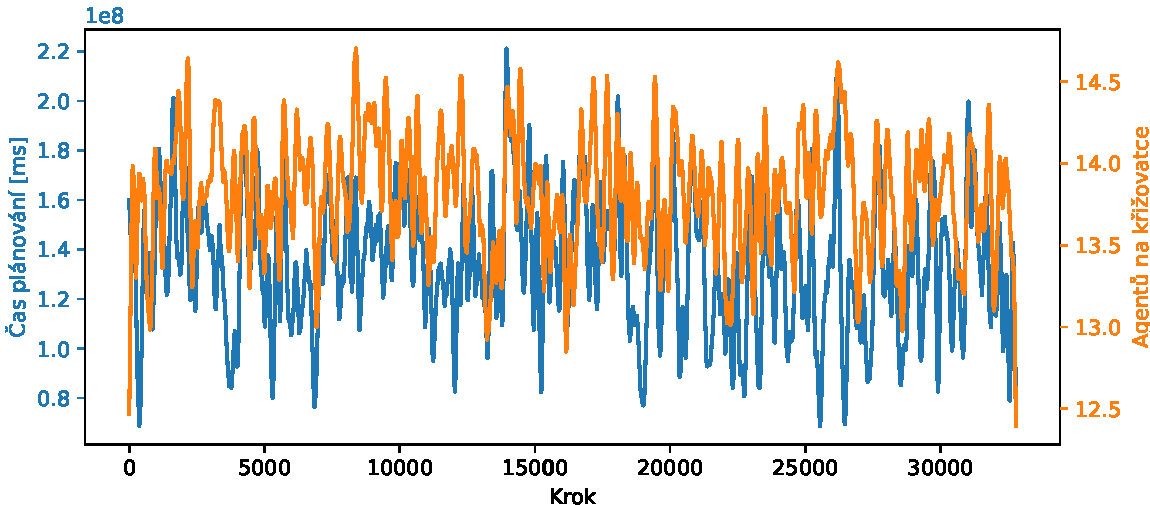
\includegraphics[width=140mm]{../img/CasVsAgentiSATRSG}
	\caption{Plánovací časy a počet naplánovaných agentů u \nameref{subsec:sat_rsg}}
	\label{fig:cas_vs_agenti_satrsg}
\end{figure}

Vytvořil jsem graf i pro \nameref{subsec:sat_ra} (Obrázek \ref{fig:cas_vs_agenti_satra}).
Tento běh byl taktéž z oktagonální křižovatky, kde algoritmus měl povolené zastavování,
\ref{str:ars_mnv} nastavené na $1$, \ref{str:ars_mpc} na $10$ a maximální počet plánovaných agentů byl $8$.

Dle mého názoru má zde mnohem větší vliv na plánování hledání modelu řešičem,
a proto je zde mnohem jasnější závislost mezi počtem agentů na křižovatce a časy plánování.
Obzvláště je zde vidět přibližně čtyřnásobná doba plánování v prvních krocích oproti průměrnému času.


\begin{figure}[h]
	\centering
	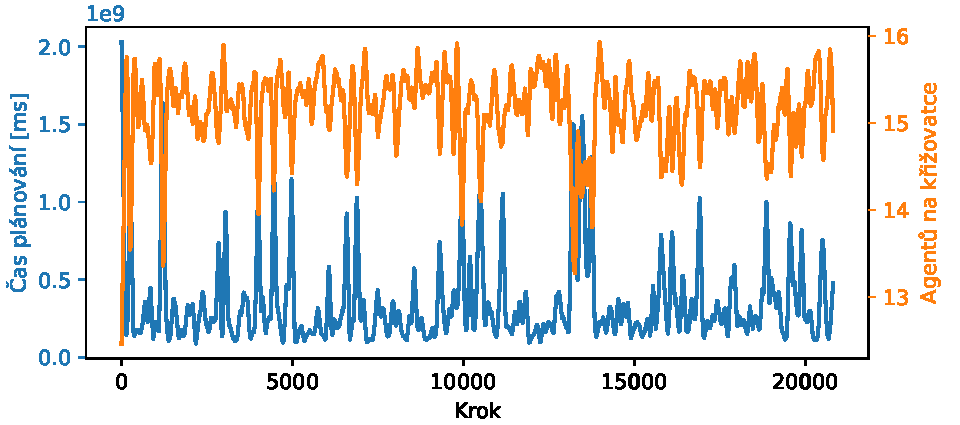
\includegraphics[width=140mm]{../img/CasVsAgentiSATRA}
	\caption{Plánovací časy a počet naplánovaných agentů u \nameref{subsec:sat_ra}}
	\label{fig:cas_vs_agenti_satra}
\end{figure}



\section{Hromadné výsledky}\label{sec:hromadne_vysledky}

Porovnání algoritmů mezi sebou s nejlepšími parametry.

Porovnání čtvercové a oktagonální křižovatky.


%\section{Neoptimální agenti}\label{sec:neoptimalni_agenti}

%Vzájemné porovnání algoritmů při datech, kdy křižovatka má nepřesná data o agentech.
